\chapter*{Der Campus++}
\addcontentsline{toc}{chapter}{Der Campus++ \hspace*{.1cm} \keys{must read}}

Auch wenn der Eine oder Andere sich das vielleicht wünscht, wird sich nicht das gesamte Studium in einem Gebäude abspielen.
Stattdessen gibt es einige wichtige Gebäude, die in deinem Studienalltag eine Rolle spielen werden.

\begin{figure}[b!]
    \centering
    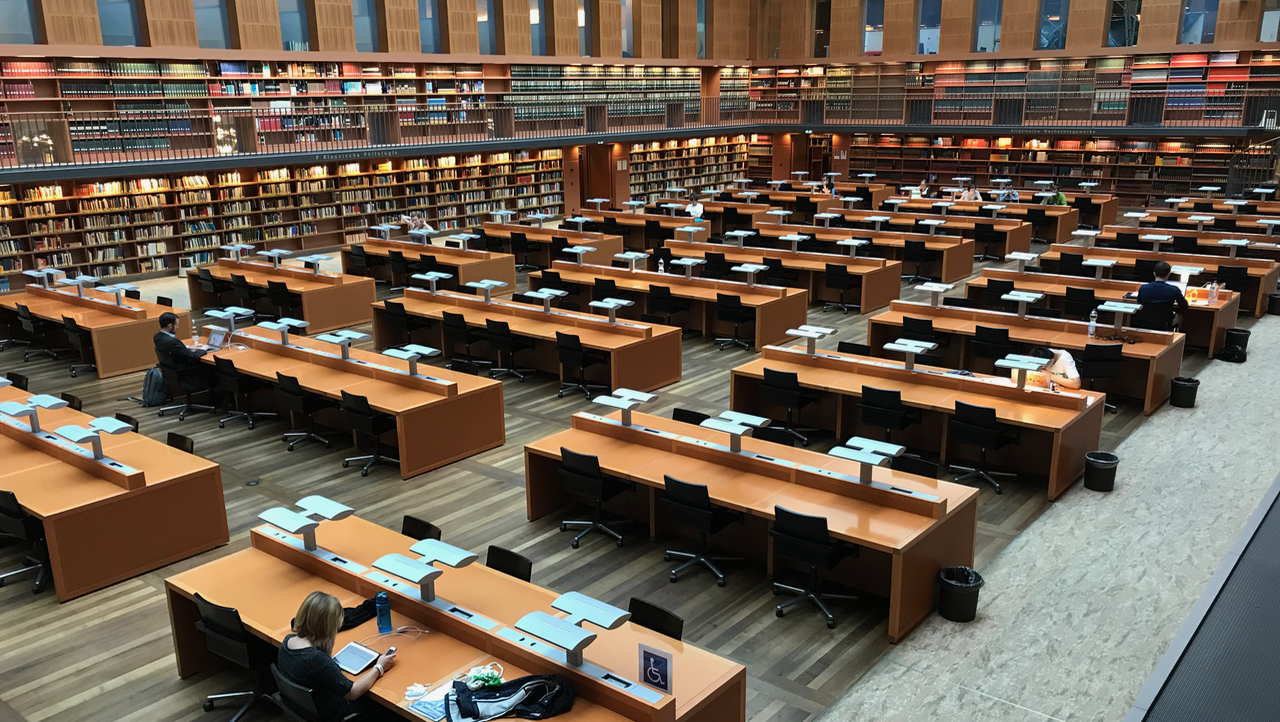
\includegraphics[width=\linewidth]{img/slub-lesesaal}
\end{figure}

\minisec{SLUB}
Die Sächsische Landesbibliothek – Staats- und Universitätsbibliothek Dresden, kurz \emph{SLUB}~\link{https://slub-dresden.de} ist das, was an anderen Universitäten einfach Bib heißt.
Mit einer Auswahl von über 12 Millionen Bestandseinheiten bestehend aus Büchern, Magazinen, Filmen, etc.\ ist sie eine der größten (Universitäts-)Bibliotheken Deutschlands.
Neben haptisch erlebbarem Lesewerk bietet die SLUB auch eine umfangreiche Auswahl online verfügbarer Ressourcen, die du dir als Studierender kostenfrei herunterladen kannst.
Viele der Bücher, die euch in Grundlagenvorlesungen empfohlen werden, hat die SLUB in großen Stückzahlen vorrätig. Ein Gang in die Lehrbuchabteilung kann euch also viele unnötige Kosten ersparen.
Gegenüber vom Hauptgebäude, dessen Lesesaal im 2. Untergeschoss ihr auf dem Bild seht, liegt die DrePunct, eine Zweigstelle der SLUB, in der die meisten Informatik-Fachbücher lagern.
Doch auch für notorische Nichtleser ist die SLUB aufgrund der vielen ruhigen Arbeitsplätzeein beliebter Aufenthaltsort.
Willst du mit Anderen gemeinsam lernen, gibt es dafür einen weiträumigen Eingangsbereich mit Gruppentischen.
Darüber hinaus können private Gruppenräume reserviert werden. Ein schönes Café, in dem per Mensakarte bezahlt werden kann, rundet das Ganze ab.
Vom APB aus befindet sich die Bibliothek jedoch am anderen Ende des Campus, was aber für Studienanfänger oft kein Problem darstellt. Denn\dots

\minisec{HSZ}
\dots\ gerade die Grundlagenvorlesungen finden nicht im APB, sondern im Hörsaalzentrum (\emph{HSZ}) statt.
In diesem, im Vergleich zum APB doch sehr eintönigen Gebäude, wirst du viele Vorlesungen zu den Grundlagen der Informatik erleben und beim Pendeln zwischen APB und HSZ den einen oder anderen Kilometer ansammeln.
Das HSZ umfasst vier Vorlesungssäle, unter Anderem das Audimax, den größten Hörsaal der Universität und das größte Auditorium Sachsens.
Zusätzlich finden sich hier noch einige Seminarräume, in welchen Übungen stattfinden können. Vor dem \enquote{zentralen Kubus} steht meist ein Mensawagen für den kleinen Hunger zwischendurch.
Auf der anderen Seite des Gebäudes ist die schöne Wiese des HSZ Veranstaltungsort für Feste oder Messen.
Zudem findest du dort den Grillcube, der dich für die Pausen zwischen Vorlesungen mit Burgern versorgt.

\minisec{Mensen}
Wer sein Studium nicht mit Pizzabestellungen bestreiten will, muss das zum Glück auch nicht, denn das Studentenwerk betreibt ein Netz aus 18 Mensen.
Egal in welchem Gebäude der Universität du dich befindest, in der Nähe wird eine Mensa oder zumindest ein Café zu finden sein.
Die Größte der Mensen, die Alte Mensa, befindet sich glücklicherweise direkt zwischen Fakultät und HSZ\@.
Hier findest du eine Vielzahl an täglich wechselnden Hauptgerichten, Salaten und Nachspeisen.
Das Tagesangebot aller Mensen ist auf der Seite des Studierendenwerks \link{https://www.studentenwerk-dresden.de/mensen/speiseplan/} zu finden.
Für Freunde des späten Frühstücks, oder Studierende mit gestörtem Schlafrhythmus findet sich in der Alten Mensa Mo-Do bis 20 Uhr ein warmes Abendangebot.
Die Auswahl ist jedoch nach 15 Uhr zunehmend eingeschränkter.
Da die Mensa zu Stoßzeiten der Fülle an Menschen kaum standhalten kann, bieten sich Essenszeiten an, die \emph{nicht} direkt nach Ende einer Doppelstunde beginnen.

Sollte euch das Angebot der Alten Mensa nicht zusagt, könnt ihr den Fußweg von 15 Minuten gern in Kauf nehmen. Das Zeltschlösschen ist eine klassische Mensa, die der Alten Mensa in so ziemlich allen Punkten unterlegen ist.

In 15 min zu Fuß könnt ihr ebenfalls die Bio-Mensa U-Boot erreichen. Der Name ist hier Programm und die, in dieser Mensa verwendeten, Zutaten sind aus biologischer und lokaler Erzeugung.
Das in der Mensa U-Boot verwendete Fleisch kommt direkt aus dem Westen Dresdens, was den Preis der Mahlzeiten allerdings nicht unerheblich erhöht.
Wählt ihr die fleischlose Alternative, sollten sich die Preise nicht sonderlich von denen anderer Mensen unterscheiden.

Auch am Wochenende kannst du dem Kochen entkommen, denn die Mensa Siedepunkt hat auch an Samstagen und Sonntagen geöffnet.
Gerade nach einer produktiven Lerneinheit in der SLUB ist diese ganz bequem mit einem einfachen Wechsel der Straßenseite zu erreichen.

\paragraph{FSR Geheimtipp:}
Ohne Zweifel die beliebteste Mensa auf dem Campus, schenkt man den Aussagen Dresdner FSRlingen glauben, ist Firat.
Es handelt sich hierbei um einen unabhängigen Dönerladen, doch durch den effizienten Umgang mit überdurchschnittlich hohem studentischen Andrang wird er gern auch scherzhaft als Mensa bezeichnet.
Das Dönerhaus liegt knapp 10 Minuten Fußweg vom APB entfernt und lockt mit guter Qualität, gemündlichem Ambiente und einer vergleichsweise großen Auswahl an Gerichten.

\minisec{Seminargebäude}
Im Seminargebäude, an der besonders schönen Fassade erkennbar, finden die Sprachkurse des LSK statt.
Für alle, die über einen einfachen Sprachkurs hinausgehen wollen, werden zusätzlich Seminare zur Kultur und Politik ausgewählter Länder und Regionen angeboten.
Weitere Informationen findest du auf der Website des LSK~\link{https://tu-dresden.de/gsw/slk/lsk}.
Das Gebäude steht direkt neben der SLUB, ca.\ 20 Minuten vom APB entfernt.

\minisec{Willersbau}
Der Willersbau~\link{https://navigator.tu-dresden.de/etplan/wil/00} ist das Gebäude der Mathematik an der TU Dresden. Hier finden teilweise eure Matheübungen statt. Der Willersbau ist in direkter Umgebung
des Hörsaalzentrums und des Trefftzbaus, in denen die Vorlesungen stattfinden. 

\minisec{Trefftzbau}
Hier~\link{https://navigator.tu-dresden.de/etplan/tre/00} finden teilweise eure Mathevorlesungen statt. Vor dem Trefftzbau befindet sich die Trefftzwiese, die gerade im Sommer wunderbar zum Entspannen nach
einer Vorlesung einlädt. 

\minisec{Studentenklub Count Down}

\begin{wrapfigure}{l}{3.25cm}%
  \vspace{-.5cm}
  
\includegraphics[width=\linewidth]{img/countdown}
  \vspace{-1cm}
\end{wrapfigure}

Wir, der Studentenklub IZ e.V., haben in den Tiefen des Wohnheims Güntzstraße 22, in der Dresdner Johannstadt unseren kleinen Studentenklub, das Count~Down~\link{https://www.countdown-dresden.de}.
IZ das steht für Informatikzentrum und tatsächlich sind wir der letzte Rest der Informatikfakultät in der Johannstadt, wo sie bis in die Mitte der 2000er ihre Heimat hatte.

Gemeinsam kochen wir, schauen Filme, zocken die Nächte durch, helfen uns gegenseitig durchs Studium oder treffen uns einfach nur so zu einer kleinen Runde Dart.
Außerdem gestalten wir zusammen als Mitglieder für dich den Rahmen unserer kleinen Bar in der Johannstadt.
Von der Auswahl der besten Biere und der leckersten Mate über die inhaltliche Gestaltung der verrücktesten Veranstaltungen und dem Mixen der absurdesten Cocktails an der Bar, bis hin zur Verschönerung des Clubs führen wir alles ehrenamtlich durch.
Dabei werden alle Entscheidungen demokratisch unter Einbezug der Kenntnis der erfahrenen Mitglieder und der frischen Ideen neuer Leute getroffen.

Zu unseren derzeitigen Veranstaltungen gehören bspw. Spieleabende, verschiedene Metalpartys, der gemeinsame Erasmus-Länderabend mit der ESN-Initiative der TU-Dresden, Werewolf- oder Cocktailabende.

\begin{wrapfigure}{r}{3.25cm}%
  %\vspace{-.5cm}
  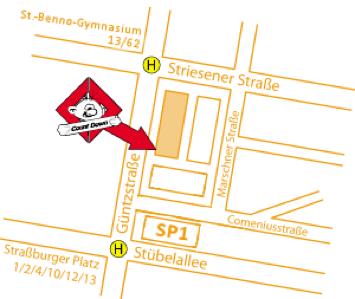
\includegraphics[width=\linewidth]{img/cd-anfahrt}
  \vspace{-1cm}
\end{wrapfigure}

Sind als nächstes auch deine tollen Ideen dabei?
Wir freuen uns immer über Nachwuchs und frische Ideen.
Komm bei uns vorbei und sprich uns an der Bar an, schreib uns eine E-Mail~\link{mailto:cd@iz-ev.de} oder bei Facebook~\link{https://www.facebook.com/countdowndd} und einer Mitgliedschaft steht nichts im Weg.
Auch die Arbeit hinter der Bar haben wir bisher noch jedem beibringen können.

\begin{awesomeblock}[ese_bg_color]{2pt}{\faCalendar*[regular]}{ese_bg_color}
    \textbf{Öffnungszeiten:}
    \begin{itemize}[noitemsep]
        \item Mo: 19:00 – 0:00
        \item Di: 20:00 – 1:00
        \item Mi: 19:00 – 0:00
        \item sowie ausgewählte Samstage
        \vspace*{-\baselineskip}
    \end{itemize}
\end{awesomeblock}
